\subsection{Aufbau} % (fold)
\label{sub:aufbau}

	\begin{figure}[H]
		\center
		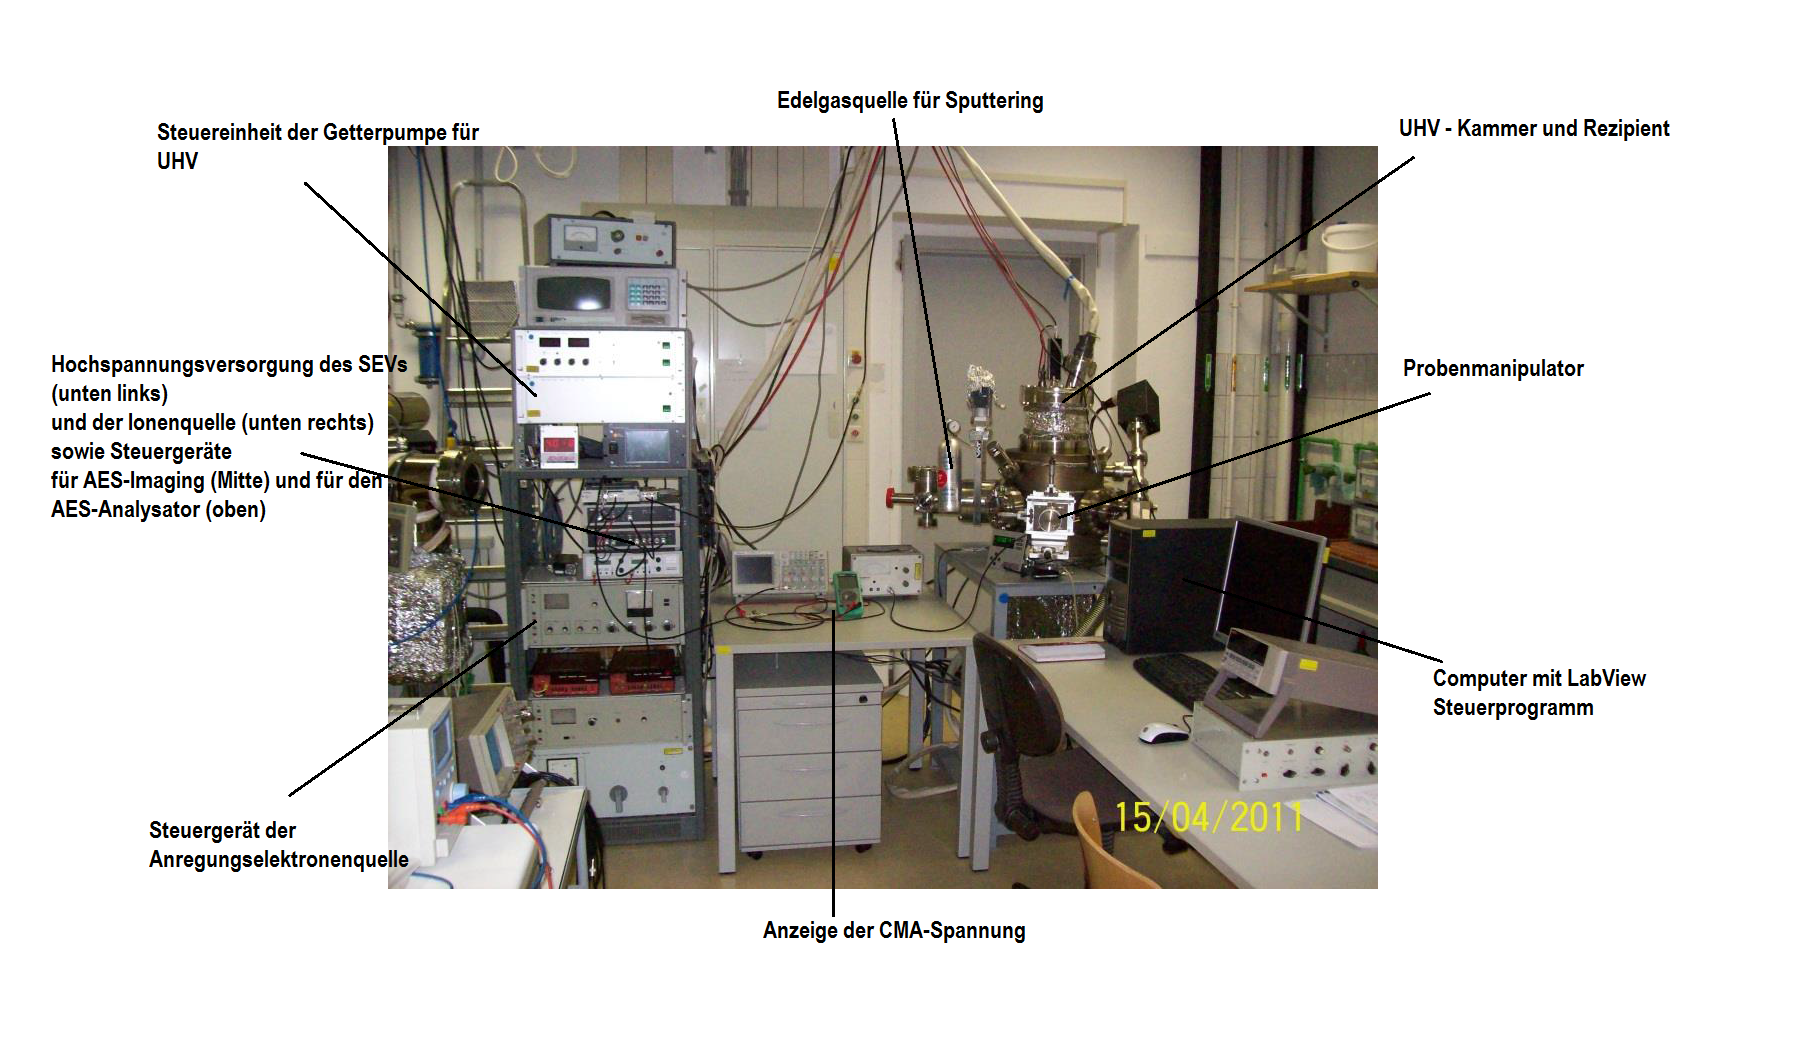
\includegraphics[scale = 0.4]{Versuchsaufbau.png}
		\caption{Aufbau nach \cite{description}}
	\end{figure}

% subsection aufbau (end)

\subsection{Durchführung} % (fold)
\label{sub:durchf_hrung}

	Das Ultrahochvakuum im Rezipienten wird mit Hilfe zweier Pumpen erzeugt. 
	Die erste Pumpe arbeitet mechanisch und erzeugt Drücke im Hochvakuumbereich. 
	Für UHV (also $10^{-10}$mbar und besser) wird dann eine Ionengetterpumpe verwendet und zudem die gesamte Anlage mehrere Tage bei 150 - 400°C ausgeheizt. \cite{description}\\

	Die Ermittlung der kinetischen Energie der rückgestrahlten Elektronen erfolgt über einen CMA (cylindrical mirror analyser). 
	Dieser besteht aus einen Zylinderkondensator mit zwei sehr kleinen Blenden am oberen und unteren Ende und lässt nur Elektronen einer bestimmten Geschwindigkeit passieren. 
	Diese treffen dann auf den Sekundärelektronenverstärker und erzeugen ein Signal.

	\begin{figure}[H]
		\center
		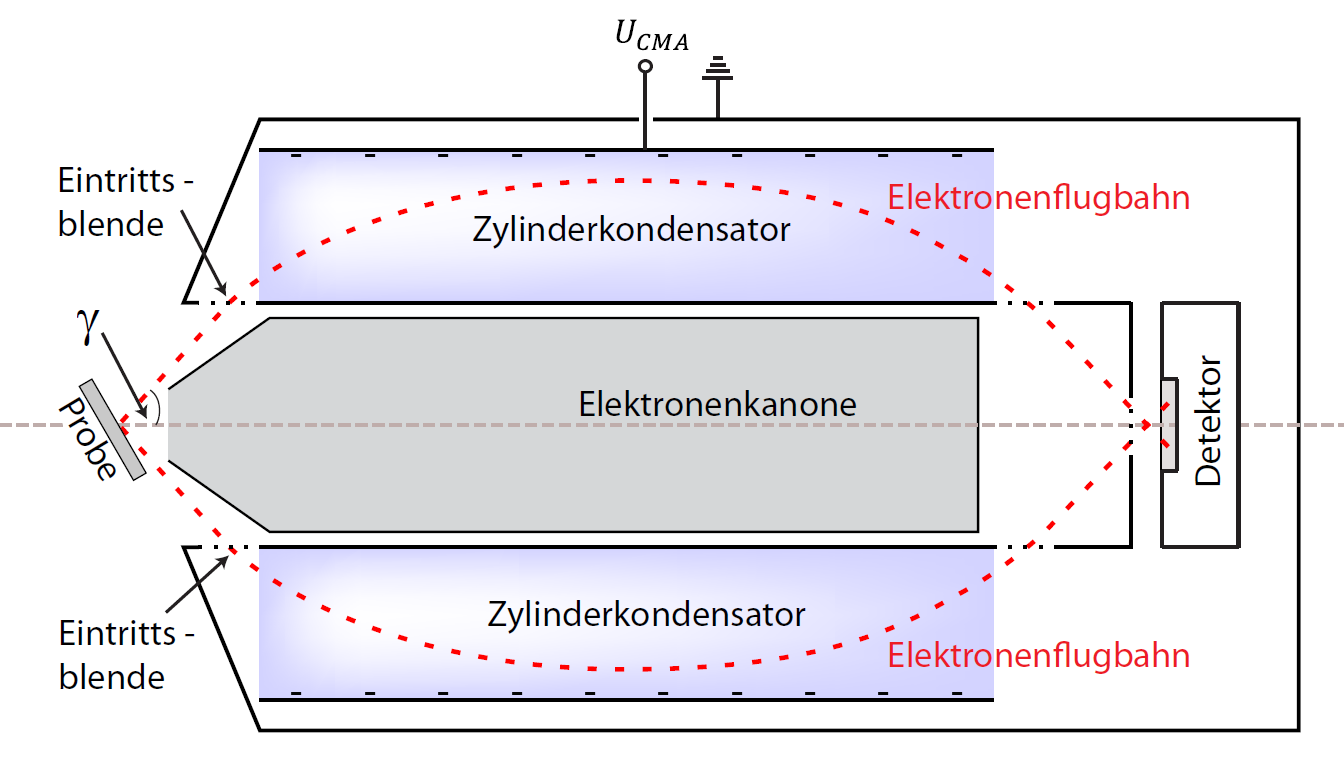
\includegraphics[scale=0.3]{cma.png}
		\caption{CMA-Aufbau nach \cite{description}}
	\end{figure}

	Da die Auger-Peaks zwar sehr scharf, aber relativ schwach im Vergleich mit Untergrund und elastischem Peak sind, empfiehlt es sich, das differentielle Spektrum zu betrachten. 
	Dieses wird mit Hilfe eines Lock-In-Verstärkers in folgender Schaltung erzeugt:

	\begin{figure}[H]
		\center
		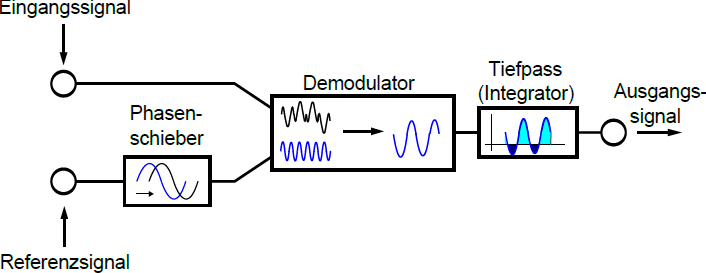
\includegraphics[scale=0.55]{lockin.png}
		\caption{Schema eines Lock-In nach \cite{description}}
	\end{figure}

	Die hochfrequente Modulationsspannung $U_{mod}$ wird dabei der Sägezahnspannung $U_{CMA}$ aufaddiert. 
	Das so gemessene Energiespektrum wird anschließend im Demodulator mit einem Referenzsignal gleicher Frequenz wie $U_{mod}$ multipliziert und über einen Tiefpass veränderlicher Zeitkonstante integriert. 
	Am Ende erhält man das Spektrum in differentieller Form.

% subsection durchf_hrung (end)